\documentclass[11pt]{article}

% Change "review" to "final" to generate camera-ready version, or "preprint" for arXiv/distribution.
\usepackage[preprint]{acl}

% Standard package includes
\usepackage{times}
\renewcommand{\ttdefault}{cmtt}
\usepackage{latexsym}
\usepackage[T1]{fontenc}
\usepackage[utf8]{inputenc}
\usepackage{microtype}
\usepackage{graphicx}
\graphicspath{{images/}{kt_survey/images/}{./}}

% Mathematical typesetting, tables, and algorithms
\usepackage{amsmath}
\usepackage{amssymb}
\usepackage{booktabs}
\usepackage{url}
\usepackage{hyperref}

\title{Tracking the Student Mind: A Comprehensive Survey and Benchmark of Deep Knowledge Tracing Paradigms, Interpretability, and Deployment Trade-Offs}

\author{Amirbek Abdirasulov \\ CSE @ UNIST\\
  \texttt{amiracle@unist.ac.kr} \\}


\begin{document}
\maketitle

\begin{abstract}
Knowledge Tracing (KT) dynamically tracks student cognitive mastery over time by modeling historical sequences of exercise attempts. Over the past decade, the field has undergone a rapid paradigm shift. Researchers progressed from classical Bayesian Hidden Markov Models to recurrent neural networks, memory-augmented matrices, self-attentive Transformers, and cognitive dual-process architectures. However, modern research has overwhelmingly prioritized leaderboard predictive accuracy (AUC). This focus often obscures fundamental trade-offs in pedagogical interpretability, cognitive plausibility, and real-time systems deployability.

In this survey and benchmark, we present a comprehensive and self-contained deconstruction of the deep knowledge tracing landscape alongside our proposed dual-process cognitive architecture, \textsc{SynapseKT}. Adopting the structural and conceptual framework of attentive knowledge tracing models, we: (1) systematically categorize the core architectural paradigms and trace their evolutionary lineage; (2) deconstruct their mathematical mechanics by contrasting monolithic hidden states, memory addressing, query-key attention, Rasch psychometric embeddings, and our proposed \textsc{SynapseKT} dual-stream fusion; (3) conduct an empirical benchmark of 20 model configurations across 6 canonical educational datasets (390 controlled experimental runs) spanning four distinct learning regimes; (4) detail our hardware workstation and software runtime to ensure full reproducibility; and (5) analyze trade-offs between predictive accuracy, cognitive interpretability (such as DKT non-monotonic ``waviness'' and memory slot collisions), parameter scaling under item sparsity, and single-step inference latency under production Intelligent Tutoring System (ITS) constraints ($\le 10$ ms). Our findings provide practical deployment guidelines and outline directions in cognitive and LLM-augmented student modeling.
\end{abstract}

\section{Introduction}
\label{sec:intro}

Personalized education systems and Intelligent Tutoring Systems (ITS) adapt instructional sequences to each student's evolving latent knowledge~\citep{corbett1994knowledge,piech2015deep}. At the core of these platforms lies \textbf{Knowledge Tracing (KT)}: estimating a student's mastery of academic concepts over time from their sequential exercise history. Accurate knowledge tracing allows instructional systems to recommend adaptive practice problems tailored to current student readiness, flag confusion loops, and schedule spaced reviews before foundational skills fade.

\begin{figure*}[t]
\centering
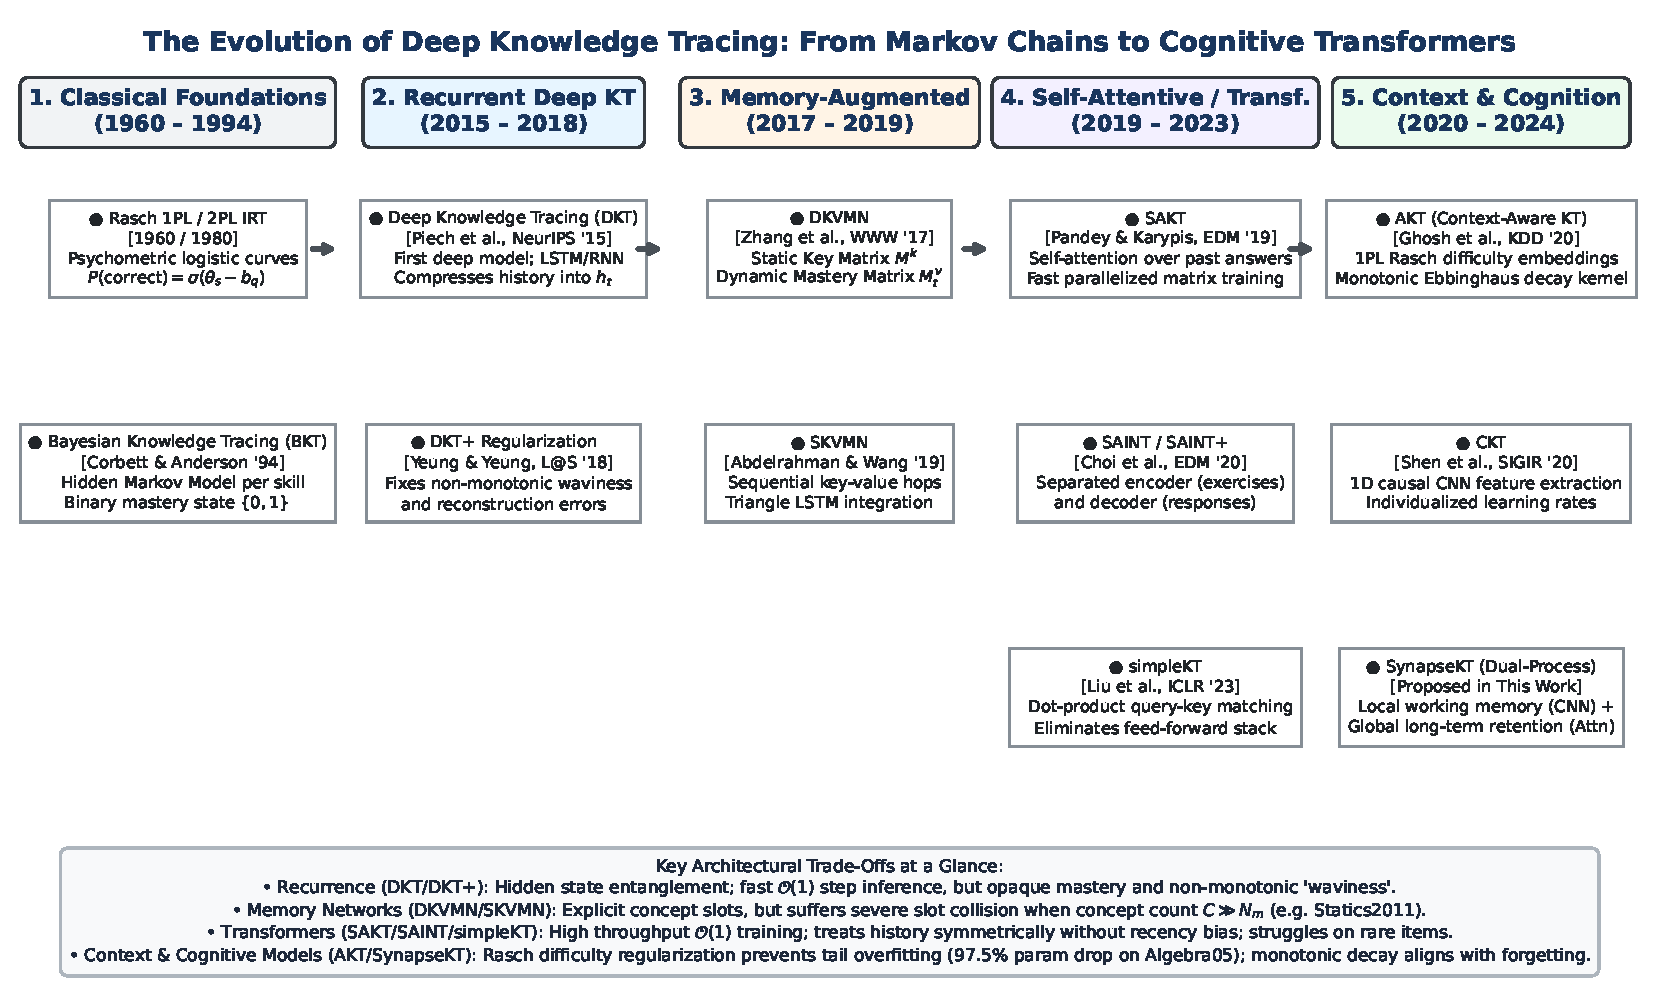
\includegraphics[width=0.98\textwidth]{fig1_kt_landscape.pdf}
\caption{\textbf{The Evolutionary Landscape of Deep Knowledge Tracing from 1994 to 2024.} Progression from classical probabilistic models (BKT, IRT) to recurrent neural networks (\textsc{DKT}, \textsc{DKT+}), dynamic memory architectures (\textsc{DKVMN}, \textsc{SKVMN}), self-attentive Transformers (\textsc{SAKT}, \textsc{SAINT}, \textsc{simpleKT}), context-aware monotonic attention (\textsc{AKT}), and our proposed dual-process cognitive hybrid (\textsc{SynapseKT}).}
\label{fig:kt_landscape}
\end{figure*}

\subsection{Formal Problem Formulation}
We formalize the Knowledge Tracing task as a sequential supervised learning problem. 

Suppose a student interacts with an educational platform over $t$ discrete time steps. At each time step $\tau \in \{1, \dots, t\}$, the student is presented with an exercise item $q_\tau \in \mathcal{Q} = \{1, \dots, Q\}$. This item is tagged with one or more underlying concepts or Knowledge Components (KCs) $c_\tau \in \mathcal{C} = \{1, \dots, C\}$. The student submits an answer, yielding a binary response outcome $r_\tau \in \{0, 1\}$. Here, $r_\tau = 1$ denotes a correct answer and $r_\tau = 0$ denotes an incorrect answer.

The student's cumulative learning history up to step $t$ is recorded as an interaction tuple sequence:
\begin{equation}
\mathcal{X}_t = \{(q_1, c_1, r_1), (q_2, c_2, r_2), \dots, (q_t, c_t, r_t)\}
\end{equation}
Given this chronological trajectory $\mathcal{X}_t$ and a candidate next exercise $(q_{t+1}, c_{t+1})$, the goal of Knowledge Tracing is to predict the probability that the student will answer correctly:
\begin{equation}
\hat{p}_{t+1} = P(r_{t+1} = 1 \mid q_{t+1}, c_{t+1}, \mathcal{X}_t)
\end{equation}

\subsection{Core Limitations of Prior Architectures}
Historically, researchers have proposed multiple families of models to solve this problem, yet each presents fundamental trade-offs:

\begin{enumerate}
    \item \textbf{Classical Markovian Baselines (BKT):} Bayesian Knowledge Tracing \citep{corbett1994knowledge} models student mastery via independent two-state Hidden Markov Models for each distinct concept. While highly interpretable, BKT assumes that different concepts are completely decoupled. It fails to capture transfer learning across prerequisite skills, such as how mastering fractions helps a student learn ratios.
    \item \textbf{Recurrent Sequence Models (DKT, DKT+):} Deep Knowledge Tracing \citep{piech2015deep} revolutionized the field by employing Long Short-Term Memory (LSTM) networks to encode the entire student trajectory into a continuous hidden state $h_t \in \mathbb{R}^d$. However, compressing all concepts into a single vector causes severe \textbf{hidden state entanglement}. Updating the hidden state after a student solves a geometry problem can inadvertently overwrite and distort the model's estimate of their algebra ability. Furthermore, DKT suffers from non-monotonic ``waviness'' \citep{yeung2018addressing}. In this pathology, answering a problem correctly counter-intuitively decreases the model's predicted mastery on that exact same problem.
    \item \textbf{Memory-Augmented Networks (DKVMN, SKVMN):} Dynamic Key-Value Memory Networks \citep{zhang2017dynamic} introduced explicit memory matrices. A static key matrix stores concept embeddings, while a dynamic value matrix stores student mastery. This mitigates hidden state entanglement, but it introduces a structural capacity bottleneck. An educational curriculum may contain hundreds or thousands of concepts ($C \gg N_m$). When the model stores them in a fixed number of memory slots (such as $N_m = 30$), it causes severe \textbf{memory slot collisions} in which unrelated concepts overwrite one another's memory cells.
    \item \textbf{Standard Self-Attention (SAKT, SAINT):} Adopting the Transformer architecture \citep{vaswani2017attention}, models such as SAKT \citep{pandey2019self} and SAINT \citep{choi2020towards} utilize multi-head self-attention to relate past exercises to the query exercise. However, standard self-attention treats all past interactions symmetrically regardless of time. In human cognition, learning decays over time according to exponential forgetting curves \citep{ebbinghaus1885memory}. Moreover, allocating dense embedding vectors for every individual exercise leads to severe overfitting when a platform contains tens of thousands of rarely attempted items.
\end{enumerate}

\subsection{Modern Attentive \& Cognitive Solutions}
Recent attentive architectures reconcile these trade-offs by incorporating two domain-specific inductive biases: psychometric Rasch embeddings and context-aware monotonic attention. Whereas standard models assign an unconstrained $d$-dimensional embedding vector to each of $100,000+$ exercises, modern models \citep{ghosh2020context,liu2023simplekt} decompose exercise representations using 1-Parameter Logistic (1PL) Rasch formulations, combining a shared concept vector with a scalar exercise difficulty parameter ($\mu_q \in \mathbb{R}$). This reduces item-level parameter counts by over 97\% while improving generalization on rarely attempted tail items. In parallel, to reflect the temporal decay of human memory \citep{ghosh2020context}, context-aware attention weights are modulated by learned exponential decay kernels ($\exp(-\theta_h \cdot \text{distance})$), aligning sequence aggregation with cognitive forgetting curves while preserving long-term associative recall. Building on these two principles, we also introduce \textbf{\textsc{SynapseKT}} in this work, a dual-process cognitive architecture that pairs multi-scale causal convolutions for working memory with adaptive monotonic attention and 2-Parameter Logistic (2PL) item discrimination.

\subsection{Contributions of this Survey}
In this paper, we connect sequence modeling, psychometrics, and educational systems engineering through the following contributions:
\begin{itemize}
    \item \textbf{Systematic Architectural Taxonomy and Unified Formulations:} We organize the deep KT landscape into seven paradigms from 1994 to 2024 (Figure~\ref{fig:kt_landscape}) and formulate recurrent transitions, dynamic memory addressing, multi-head attention, Rasch difficulty regularizations, and our proposed \textsc{SynapseKT} dual-process model within a unified mathematical notation.
    \item \textbf{Unified 20-Model Master Benchmark:} We evaluate 20 model configurations (19 established baselines plus our proposed \textsc{SynapseKT} architecture) across 6 canonical datasets (390 controlled experimental runs) using strict 5-fold student-level cross-validation across four educational regimes.
    \item \textbf{Multi-Dimensional Trade-Off Analysis:} We analyze the trade-offs between predictive accuracy (AUC), model interpretability, parameter scaling on sparse catalogs, and real-time single-step inference latency under Intelligent Tutoring System production Service Level Agreements ($\le 10$ ms), and synthesize actionable deployment guidelines.
    \item \textbf{Open-Source Software Framework (\texttt{ktbench}):} We document our hardware execution environment and release the complete software framework developed for this benchmark at \url{https://github.com/mirabdi/KT} \citep{abdimutalipov2024ktbench}, featuring modular PyTorch 2.x implementations, automated data adapters, and unit test coverage.
\end{itemize}

% =============================================================================
\section{Evolution of the Knowledge Tracing Landscape}
\label{sec:landscape}
% =============================================================================

The knowledge tracing landscape has evolved across five distinct epochs, transitioning from discrete psychometric models to modern cognitive transformers.

\subsection{Classical Psychometrics and BKT (1960 to 1994)}
Prior to deep learning, student modeling relied on two foundational frameworks: Item Response Theory (IRT) and Bayesian Knowledge Tracing (BKT). Developed in educational measurement \citep{rasch1960probabilistic,lord1980applications}, IRT models the probability of a correct response as a logistic function of student latent ability $\theta_s \in \mathbb{R}$ and item difficulty $b_q \in \mathbb{R}$:
\begin{equation}
P(r_{s,q} = 1) = \sigma(\theta_s - b_q)
\end{equation}
where $\sigma(z) = (1 + \exp(-z))^{-1}$. In the 2-Parameter Logistic (2PL) extension, a discrimination parameter $\alpha_q > 0$ scales the item's ability to differentiate between high- and low-performing students: $P(r_{s,q} = 1) = \sigma(\alpha_q(\theta_s - b_q))$. While IRT provides strong psychometric construct validity, it is static and assumes that a student's ability $\theta_s$ remains constant during an assessment.

To capture learning dynamics over time, \citet{corbett1994knowledge} introduced BKT, which models student mastery of each individual concept as a Hidden Markov Model (HMM) with binary states: unmastered ($L_t = 0$) or mastered ($L_t = 1$). BKT is governed by four parameters per skill: initial mastery $P(L_0)$, transition probability $P(T) = P(L_{t+1}=1 \mid L_t=0)$, slip probability $P(S) = P(r_t=0 \mid L_t=1)$, and guess probability $P(G) = P(r_t=1 \mid L_t=0)$. Because BKT fits independent parameters for each concept, it does not capture cross-skill transfer or prerequisite correlations.

\subsection{Deep Recurrent Models: DKT and DKT+ (2015 to 2018)}
The deep learning revolution in educational data mining began with \textbf{Deep Knowledge Tracing (\textsc{DKT})} \citep{piech2015deep}. Instead of discrete Markovian states, DKT utilizes a Long Short-Term Memory (LSTM) network or Elman Recurrent Neural Network (RNN) to track student cognitive state continuously.

At each step $t$, the student interaction $(c_t, r_t)$ is encoded as a one-hot vector $x_t \in \{0, 1\}^{2C}$. The first $C$ dimensions indicate answering concept $c_t$ incorrectly ($r_t = 0$). The second $C$ dimensions indicate answering correctly ($r_t = 1$). The recurrent hidden state updates via:
\begin{equation}
h_t = \text{LSTM}(x_t, h_{t-1})
\end{equation}
The predicted probability of answering any concept $k \in \{1, \dots, C\}$ correctly at step $t+1$ is computed by projecting $h_t$ through a sigmoid output layer:
\begin{equation}
\hat{y}_{t+1} = \sigma(W_{out} h_t + b_{out}) \in (0, 1)^C
\end{equation}
The predicted probability for the query concept $c_{t+1}$ is then indexed directly: $\hat{p}_{t+1} = \hat{y}_{t+1}[c_{t+1}]$.

\paragraph{DKT+ Consistency Regularization.}
Although DKT substantially improved predictive accuracy over BKT, \citet{yeung2018addressing} identified two structural pathologies in recurrent representations: \emph{non-monotonic waviness}, wherein predicted performance on unpracticed concepts oscillates erratically due to entangled hidden state updates, and \emph{reconstruction inconsistency}, where correctly answering a problem at step $t$ can paradoxically lower the model's updated prediction $\hat{y}_{t+1}$ on that same item. To penalize these artifacts, \citet{yeung2018addressing} introduced \textsc{DKT+}, augmenting the cross-entropy loss $\mathcal{L}_{CE}$ with two consistency regularizers:
\begin{equation}
\mathcal{L}_{DKT+} = \mathcal{L}_{CE} + \lambda_r \mathcal{L}_{rec} + \lambda_w \mathcal{L}_{wave}
\end{equation}
Here, $\mathcal{L}_{rec}$ penalizes predictions that contradict the immediate observation, and $\mathcal{L}_{wave}$ penalizes large fluctuations across consecutive steps for unpracticed concepts.

\subsection{Memory-Augmented Models: DKVMN and SKVMN (2017 to 2019)}
To eliminate hidden state entanglement, \citet{zhang2017dynamic} introduced \textbf{Dynamic Key-Value Memory Networks (\textsc{DKVMN})}, inspired by neural Turing machines. 

Instead of a single hidden vector, DKVMN decouples memory into two matrices: a static key matrix $M^k \in \mathbb{R}^{N_m \times d}$, whose $N_m$ slots represent latent concept embeddings shared across students, and a dynamic value matrix $M_t^v \in \mathbb{R}^{N_m \times d}$, updated after each interaction to track individual student mastery across those slots.

When presented with exercise $q_t$ (embedded as $k_t \in \mathbb{R}^d$), the model computes a softmax correlation vector over all $N_m$ memory slots:
\begin{equation}
w_t(i) = \text{Softmax}(k_t^T M^k(i))
\end{equation}
The student's current mastery state is retrieved by a weighted sum over the value matrix: $r_t = \sum_{i=1}^{N_m} w_t(i) M_t^v(i)$. After observing the response $r_t$, the value memory is updated via explicit erase and add vectors:
\begin{equation}
M_t^v(i) = M_{t-1}^v(i) \odot (1 - w_t(i) e_t) + w_t(i) a_t
\end{equation}
Subsequently, \citet{abdelrahman2019knowledge} extended this with \textbf{Sequential Key-Value Memory Networks (\textsc{SKVMN})}. SKVMN utilizes a triangle LSTM to combine hop-based memory addressing with sequential recurrence.

\subsection{Attentive Models: SAKT, SAINT, and simpleKT (2019 to 2023)}
While recurrent and memory networks must process sequences step by step, Transformers \citep{vaswani2017attention} unlocked parallel training and direct long-range credit assignment.

\paragraph{Self-Attentive Models: SAKT, SAINT, and simpleKT.}
\citet{pandey2019self} introduced Self-Attentive Knowledge Tracing (\textsc{SAKT}), using multi-head attention to evaluate historical interactions against candidate concept queries without sequential recurrence. However, SAKT concatenates exercises and responses into a single sequence, conflating the problem attempted with the student's performance outcome. To resolve this, \citet{choi2020towards} proposed \textsc{SAINT}, decoupling inputs into a separated encoder that self-attends over exercise sequences and a decoder that applies self-attention over response histories and cross-attention over exercise representations. \textsc{SAINT+} \citep{shin2021saint} further incorporated temporal features such as response latency and inter-interaction lag. More recently, \citet{liu2023simplekt} introduced \textsc{simpleKT}, demonstrating that deep Transformer stacks can be simplified into a minimalist scaled dot-product attention kernel that directly queries exercise representations, mitigating overparameterization while accelerating inference.

\subsection{Context-Aware Monotonic Attention: AKT (2020)}
\citet{ghosh2020context} proposed \textbf{Context-Aware Attentive Knowledge Tracing (\textsc{AKT})}, addressing two critical limitations of standard self-attention: the symmetric treatment of historical interactions regardless of temporal distance, and catastrophic overfitting caused by assigning independent dense embeddings to rare items in sparse catalogs. 

AKT introduces two principled mechanisms. First, question representations are grounded via 1-Parameter Logistic (1PL) Rasch psychometrics: the embedding of question $q$ decomposes into a base concept vector $c_c \in \mathbb{R}^d$ and a learned scalar item difficulty offset $\mu_q \in \mathbb{R}$:
\begin{equation}
x_q = c_c + \mu_q d_c
\end{equation}
where $d_c \in \mathbb{R}^d$ denotes a concept variation vector, regularizing tail items toward the shared concept manifold. Second, AKT modulates attention logits by an exponential decay kernel aligned with cognitive forgetting curves:
\begin{equation}
\text{Score}(t, \tau) = \frac{Q_t K_\tau^T}{\sqrt{d}} - \theta_h \cdot \text{dist}(t, \tau)
\label{eq:akt_decay}
\end{equation}
where $\theta_h > 0$ is a learnable decay parameter for attention head $h$, and $\text{dist}(t, \tau)$ represents contextual or temporal distance. This enforces cognitive recency bias while preserving relevant long-term recall.

\subsection{Convolutional and Proposed Cognitive Dual-Process Models (2020 to 2024)}
Beyond pure recurrence and attention, recent work has explored local convolutional filtering and dual-process cognitive architectures. \citet{shen2020convolutional} proposed \textbf{Convolutional Knowledge Tracing (\textsc{CKT})}, observing that student learning occurs in localized practice sessions. CKT utilizes causal 1D convolutional layers with Gated Linear Units (GLUs) to extract local response streaks (such as consecutive errors signaling confusion or fatigue) before computing global representations.

Building on these foundations, we propose \textbf{Cognitive Dual-Process Knowledge Tracing (\textsc{SynapseKT})} as part of this work. Motivated by dual-process theories of human memory \citep{baddeley1992working,kahneman2011thinking}, \textsc{SynapseKT} models student cognition through two concurrent pathways: (1) a local \textbf{Working Memory} stream that captures immediate cognitive momentum and fatigue via multi-scale causal convolutions; and (2) a global \textbf{Long-Term Memory} associative stream that tracks curriculum-wide prerequisite mastery via monotonic attention with practice-dependent consolidation decay. The two streams are dynamically combined through a learned confidence gate (detailed in Section~\ref{sec:framework}).

% =============================================================================
\section{Theoretical Framework and Mechanics}
\label{sec:framework}
% =============================================================================

To understand why different KT models perform differently across educational benchmarks, we must deconstruct their mathematical mechanics. In this section, we examine the foundational building blocks governing input representations and history summarization.

\begin{figure*}[t]
\centering
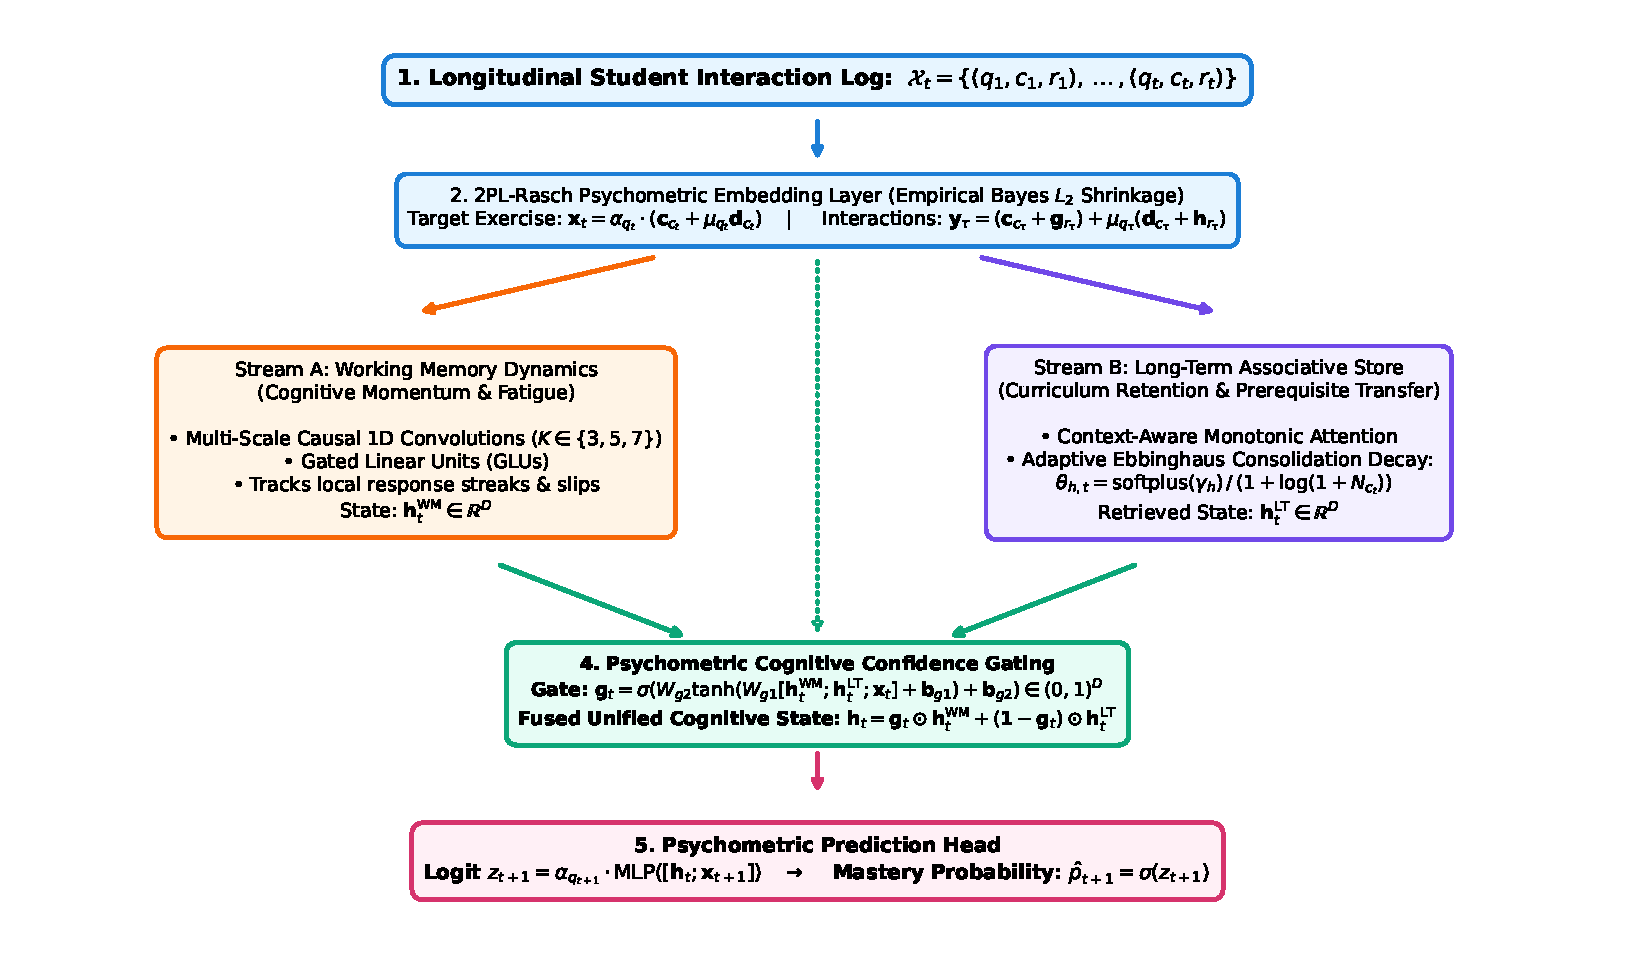
\includegraphics[width=0.92\textwidth]{fig5_synapsekt_architecture.pdf}
\caption{\textbf{Our Proposed SynapseKT Dual-Process Architecture.} Student interactions are embedded via 2PL-Rasch psychometric projections. Stream A (Working Memory) processes local streaks via causal 1D convolutions and GLUs. Stream B (Long-Term Associative Memory) retrieves curriculum mastery via context-aware monotonic attention with Ebbinghaus consolidation decay. A confidence gate dynamically fuses both streams into a final psychometric prediction logit.}
\label{fig:synapsekt_arch}
\end{figure*}

\subsection{Input Representations: The Rasch Formulation}
In any machine learning pipeline, how features are embedded into vector space determines generalization performance. 

\paragraph{Item Parameterization and the Sparsity Dilemma.}
A direct approach to representing exercises in an ITS is to assign an independent $d$-dimensional embedding vector to each question $q \in \{1, \dots, Q\}$. However, consider an educational dataset such as \textsc{Algebra2005}, which contains $Q = 173,113$ distinct question steps across $C = 112$ high-level algebra concepts. Allocating an unconstrained embedding matrix for questions with dimension $d = 128$ requires:
\begin{equation}
173,113 \times 128 \approx 22,158,464 \text{ parameters}
\end{equation}
Because exercise frequency in real-world educational platforms follows a heavy-tailed power law, a small subset of popular questions receives thousands of attempts, while tens of thousands of niche problems are attempted only once or twice. An unconstrained $22$-million parameter embedding matrix overfits heavily to rare questions, memorizing item-specific noise rather than generalizable skills.

\paragraph{Rasch Decomposition and Complexity Scaling.}
The 1-Parameter Logistic (1PL) Rasch formulation resolves this parameter explosion by decomposing item representations. Rather than allocating an unconstrained vector per question, the model learns a base concept embedding matrix $E_c \in \mathbb{R}^{C \times d}$, a concept variation matrix $E_d \in \mathbb{R}^{C \times d}$, and a single scalar difficulty parameter $\mu_q \in \mathbb{R}$ for each question item $q \in \{1, \dots, Q\}$. The vector representation $x_q \in \mathbb{R}^d$ for question $q$ under concept $c$ is computed as:
\begin{equation}
x_q = E_c[c] + \mu_q \cdot E_d[c]
\label{eq:rasch_embed}
\end{equation}
For historical interactions $(q_\tau, c_\tau, r_\tau)$, response offset vectors $g_r, h_r \in \mathbb{R}^d$ are incorporated:
\begin{equation}
y_\tau = (E_c[c_\tau] + g_{r_\tau}) + \mu_{q_\tau} \cdot (E_d[c_\tau] + h_{r_\tau})
\end{equation}
By reducing question-specific parameters from a $d$-dimensional vector to a single scalar $\mu_q$, parameter complexity shrinks from $\mathcal{O}(Q \cdot d)$ to $\mathcal{O}(C \cdot d + Q)$. On \textsc{Algebra2005}, this reduces item parameters from \textbf{22.6 Million} to \textbf{0.57 Million} (a 97.5\% reduction) while improving test-set AUC by over 4.4\%.

\subsection{History Summarization Mechanisms}
Once inputs are embedded, the model must summarize the student's historical interaction sequence $\mathcal{X}_t$ into a predictive representation. Four primary computational mechanisms govern sequence aggregation:

\subsubsection{1. Recurrent Compression (DKT)}
Recurrent models maintain a monolithic hidden state vector $h_t \in \mathbb{R}^d$, updating sequentially via:
\begin{equation}
h_t = \tanh(W_{hh} h_{t-1} + W_{xh} y_t + b_h)
\end{equation}
Here, $h_t$ operates as a lossy compressed buffer. When a student practices dozens of concepts across a curriculum, compressing all skills into a fixed-size vector induces hidden state entanglement: updating coordinates associated with concept $A$ modifies dimensions that simultaneously encode concept $B$, resulting in non-monotonic oscillations across unpracticed skills.

\subsubsection{2. Memory Addressing (DKVMN)}
Memory networks decompose the state into an array of $N_m$ explicit memory slots $M_t^v \in \mathbb{R}^{N_m \times d}$. Addressing is computed via content-based cosine similarity with key matrix $M^k$:
\begin{equation}
w_t(i) = \frac{\exp(k_t \cdot M^k(i) / \sqrt{d})}{\sum_{j=1}^{N_m} \exp(k_t \cdot M^k(j) / \sqrt{d})}
\end{equation}
The memory matrix operates as an associative hash table where memory slots serve as latent buckets. When curriculum size $C \approx N_m$, each slot maps cleanly to a small concept cluster. However, when the curriculum expands to fine-grained hierarchies ($C \gg N_m$, such as $C = 1,223$ in engineering statics), each slot must superimpose dozens of distinct skills, creating severe slot collisions and destructive overwrites.

\subsubsection{3. Multi-Head Query-Key Attention (SAKT, SAINT)}
Transformers preserve the full sequence of past embeddings $\{y_1, \dots, y_t\}$ without recurrent compression. Given target query $q_{t+1}$, the model computes attention weights across past steps $\tau \le t$:
\begin{equation}
\alpha_{t, \tau} = \text{Softmax}\left(\frac{(x_{q_{t+1}} W_Q)(y_\tau W_K)^T}{\sqrt{d_k}}\right)
\end{equation}
and aggregates context via $c_{t+1} = \sum_{\tau=1}^t \alpha_{t, \tau} (y_\tau W_V)$. While dynamic query-key retrieval prevents recurrent compression bottlenecks, standard self-attention is permutation-invariant and lacks an intrinsic recency bias: without explicit decay or positional encodings, an interaction completed weeks ago receives equal weight to an interaction completed seconds ago.

\subsubsection{4. Monotonic Exponential Decay Attention (AKT)}
To incorporate the cognitive reality of forgetting, AKT modifies the attention logits by subtracting a distance penalty:
\begin{equation}
\alpha_{t, \tau}^{(h)} = \frac{\exp\left(\frac{Q_t^{(h)} (K_\tau^{(h)})^T}{\sqrt{d_k}} - \theta_h \cdot d(t, \tau)\right)}{\sum_{\tau'=1}^t \exp\left(\frac{Q_t^{(h)} (K_{\tau'}^{(h)})^T}{\sqrt{d_k}} - \theta_h \cdot d(t, \tau')\right)}
\end{equation}
where $\theta_h > 0$ is a learnable decay parameter for head $h$, and $d(t, \tau) = \sqrt{t - \tau}$ represents temporal distance. As analyzed in Section~\ref{sec:tradeoffs}, multi-head monotonic decay enables individual heads to specialize across distinct cognitive timescales: localized heads learn steep decay to capture working memory and immediate slips, while long-term heads learn shallow decay to track foundational mastery.

\subsection{Proposed Synaptic Dual-Process Fusion (SynapseKT)}
As illustrated in Figure~\ref{fig:synapsekt_arch}, \textsc{SynapseKT} unifies local working memory and global associative memory within a dual-stream architecture:
\begin{enumerate}
    \item \textbf{Stream A (Working Memory):} Processes recent interactions via causal 1D convolutions with Gated Linear Units (GLUs), producing a local momentum state $h_t^{WM} \in \mathbb{R}^d$.
    \item \textbf{Stream B (Long-Term Associative Memory):} Retrieves historical mastery across the full curriculum via context-aware monotonic attention with consolidation decay, yielding long-term state $h_t^{LT} \in \mathbb{R}^d$.
    \item \textbf{Confidence Gating:} A learned gating mechanism dynamically balances both streams based on sequence context:
    \begin{align}
    u_t &= [h_t^{WM} ; h_t^{LT} ; x_{t+1}] \\
    g_t &= \sigma\big(W_{g2} \tanh(W_{g1} u_t + b_{g1}) + b_{g2}\big) \\
    h_t &= g_t \odot h_t^{WM} + (1 - g_t) \odot h_t^{LT}
    \end{align}
    where $g_t \in (0, 1)^d$.
    \item \textbf{2PL Psychometric Prediction:} The fused representation $h_t$ is projected through a multi-layer perceptron and scaled by the 2PL item discrimination parameter $\alpha_{q_{t+1}} > 0$:
    \begin{equation}
    \hat{p}_{t+1} = \sigma\left(\alpha_{q_{t+1}} \cdot \text{MLP}([h_t ; x_{q_{t+1}}])\right)
    \end{equation}
\end{enumerate}

% =============================================================================
\section{Empirical Evaluation and Master Benchmark}
\label{sec:experiments}
% =============================================================================

To empirically validate how these architectures perform across diverse educational contexts, we conducted an exhaustive benchmark spanning 20 model configurations and 6 canonical datasets.

\subsection{Experimental Setup}

\paragraph{Datasets and Educational Regimes:}
We evaluated all models across six widely utilized benchmarks, selected to represent four distinct operational regimes in educational technology:
\begin{enumerate}
    \item \textbf{Regime 1: Longitudinal K-12 Tutoring (\textsc{ASSISTments2009}, \textsc{ASSISTments2017}):} Long student interaction sequences collected from real-world online middle school math tutors, characterized by multi-step problem solving and progressive mastery.
    \item \textbf{Regime 2: Ultra-Sparse Massive Catalogs (\textsc{Algebra2005}):} A massive K-12 algebra problem catalog from the KDD Cup 2010 containing over 173,000 distinct question steps mapped to 112 concepts. The vast majority of questions have fewer than five attempts, creating an extreme test of model regularization and parameter efficiency.
    \item \textbf{Regime 3: High-Granularity Engineering Concepts (\textsc{Statics2011}):} Collected from a college-level mechanical engineering statics course. Characterized by a massive concept hierarchy ($C = 1,223$ fine-grained concepts) tested on a moderate student cohort.
    \item \textbf{Regime 4: Dense Diagnostic Quizzes (\textsc{NIPS34}, \textsc{ASSISTments2015}):} High-density, short-duration diagnostic tests where students answer multiple-choice diagnostic items.
\end{enumerate}

\paragraph{Strict Causality and Cross-Validation Protocol:}
To prevent data leakage, all evaluations followed strict 5-fold cross-validation partitioned strictly at the student level. All interactions for a given student belong exclusively to either the training set or the test set. Within each sequence, models predict step $t+1$ strictly conditioned on interactions $\tau \le t$, preventing future-to-past leakage.

\paragraph{Evaluation Metrics.}
We evaluate model performance using three standard metrics: Area Under the ROC Curve (AUC) as the primary threshold-independent ranking metric, Root Mean Squared Error (RMSE) to assess probability calibration ($\sqrt{\frac{1}{N}\sum (\hat{p}_i - r_i)^2}$), and classification Accuracy (ACC) evaluated at a $0.5$ decision threshold.

\subsection{Experimenting Machine and Reproducibility Environment}
\label{sec:machine_specs}
To ensure full reproducibility, all benchmark training runs, 5-fold evaluations, and latency measurements were executed on a single standardized workstation using our open-source \texttt{ktbench} library, hosted at \url{https://github.com/mirabdi/KT} \citep{abdimutalipov2024ktbench}.

\paragraph{Hardware and Software Environment:}
Experiments were conducted on an Apple MacBook Air (\texttt{Mac15,13}) equipped with an Apple M3 System-on-Chip (8-core CPU with 4 performance and 4 efficiency cores up to 4.05 GHz, 10-core integrated GPU, and 16-core Neural Engine) and 16 GB of unified LPDDR5 memory (100 GB/s bandwidth). Because the CPU and GPU share unified memory with zero-copy addressing, PCIe transfer overhead is eliminated during single-step latency profiling. The host ran macOS Sequoia 15.1 (ARM64 Darwin 24.1.0) with Python 3.12.7 and PyTorch 2.5.1 using native Metal Performance Shaders (\textsc{MPS}) acceleration, alongside Scikit-Learn 1.5.2, NumPy 2.1.2, SciPy 1.14.1, and Pandas 2.2.3.

\paragraph{The \texttt{ktbench} Benchmarking Framework:}
The open-source repository \citep{abdimutalipov2024ktbench} enforces a 4-layer decoupled design separating configuration dataclasses (\texttt{config.py}), dataset adapters (\texttt{data/}), model implementations (\texttt{models/}), and training orchestration (\texttt{training/}). To train sequence models efficiently within a 16 GB unified memory budget, the framework implements length-bucketed dynamic batching and gradient accumulation. Correctness of gradient backpropagation, causal masking, and metric calculation is verified by a suite of 53 unit and regression tests in \texttt{pytest}. All 390 experimental runs across the 20 model configurations used fixed random seeds (seed 42), and single-step inference latency was profiled across 1,000 warm iterations using monotonic wall clocks.

\begin{table*}[t]
\centering
\caption{\textbf{Master Cross-Dataset Empirical Benchmark.} 5-fold student-level cross-validation performance across 6 canonical educational datasets (390 experimental runs). All 20 model configurations are evaluated across 7 paradigm families. Bold indicates top performance per dataset; underline indicates runner-up. Dashes ($-$) indicate concept-only datasets lacking item-level question IDs where Rasch variants reduce to non-Rasch. Datasets span four distinct educational regimes: Longitudinal Tutoring (\textsc{ASSIST09}, \textsc{ASSIST17}), Ultra-Sparse Catalogs (\textsc{Algebra05}), Granular Concepts (\textsc{Statics11}), and Dense Diagnostic Quizzes (\textsc{NIPS34}, \textsc{ASSIST15}).}
\label{tab:master_benchmark}
\resizebox{\textwidth}{!}{
\begin{tabular}{llcccccccccccc}
\toprule
\textbf{Paradigm Family} & \textbf{Model Architecture} & \multicolumn{2}{c}{\textbf{ASSISTments2009}} & \multicolumn{2}{c}{\textbf{ASSISTments2015}} & \multicolumn{2}{c}{\textbf{ASSISTments2017}} & \multicolumn{2}{c}{\textbf{Statics2011}} & \multicolumn{2}{c}{\textbf{Algebra2005}} & \multicolumn{2}{c}{\textbf{NIPS34 (Task 3/4)}} \\
\cmidrule(lr){3-4} \cmidrule(lr){5-6} \cmidrule(lr){7-8} \cmidrule(lr){9-10} \cmidrule(lr){11-12} \cmidrule(lr){13-14}
& & \textbf{AUC} & \textbf{RMSE} & \textbf{AUC} & \textbf{RMSE} & \textbf{AUC} & \textbf{RMSE} & \textbf{AUC} & \textbf{RMSE} & \textbf{AUC} & \textbf{RMSE} & \textbf{AUC} & \textbf{RMSE} \\
\midrule
\textbf{Recurrent} & \textsc{DKT} (LSTM) & 0.8176 & 0.3958 & 0.7317 & 0.4127 & 0.7276 & 0.4457 & 0.8233 & 0.3668 & 0.9061 & 0.3177 & 0.7587 & 0.4450 \\
& \textsc{DKT+} (Regularized) & 0.8109 & 0.3984 & 0.7322 & 0.4126 & 0.7135 & 0.4497 & \textbf{0.8294} & \textbf{0.3638} & 0.9065 & 0.3174 & 0.7593 & 0.4447 \\
& \textsc{DKT-R} (Rasch) & 0.8189 & 0.3952 & $-$ & $-$ & 0.7606 & 0.4341 & $-$ & $-$ & 0.9183 & 0.3086 & 0.7886 & 0.4316 \\
& \textsc{DKT+-R} (Reg.\ + Rasch) & 0.8123 & 0.3978 & $-$ & $-$ & 0.7477 & 0.4387 & $-$ & $-$ & 0.9182 & 0.3090 & 0.7889 & \underline{0.4315} \\
\midrule
\textbf{Memory} & \textsc{DKVMN} & 0.8093 & 0.3993 & 0.7273 & 0.4136 & 0.7079 & 0.4512 & 0.8215 & 0.3676 & 0.9072 & 0.3172 & 0.7598 & 0.4445 \\
& \textsc{DKVMN-R} (Rasch) & 0.8247 & 0.3921 & $-$ & $-$ & 0.7572 & 0.4346 & $-$ & $-$ & 0.9185 & 0.3093 & \underline{0.7891} & 0.4316 \\
& \textsc{SKVMN} (Sequential) & 0.7084 & 0.4475 & 0.6972 & 0.4200 & 0.6486 & 0.4628 & 0.5943 & 0.4163 & 0.8143 & 0.3792 & 0.7423 & 0.4517 \\
\midrule
\textbf{Single Attn} & \textsc{SAKT} & 0.7526 & 0.4272 & 0.7227 & 0.4160 & 0.6592 & 0.4634 & 0.8015 & 0.3792 & 0.8627 & 0.3519 & 0.7446 & 0.4511 \\
& \textsc{SAKT-R} (Rasch) & 0.7750 & 0.4191 & $-$ & $-$ & 0.7067 & 0.4506 & $-$ & $-$ & 0.8810 & 0.3418 & 0.7804 & 0.4360 \\
& \textsc{simpleKT} & 0.7549 & 0.4329 & 0.6997 & 0.4194 & 0.7087 & 0.4464 & 0.6446 & 0.4060 & 0.8838 & 0.3373 & 0.7826 & 0.4334 \\
\midrule
\textbf{Separated Attn} & \textsc{SAINT} (Dense) & 0.7554 & 0.4306 & 0.6764 & 0.4248 & 0.6385 & 0.4649 & 0.5974 & 0.4137 & 0.8497 & 0.3591 & 0.7367 & 0.4540 \\
& \textsc{SAINT-R} (Rasch) & 0.7832 & 0.4194 & $-$ & $-$ & 0.7102 & 0.4468 & $-$ & $-$ & 0.8945 & 0.3307 & 0.7859 & 0.4335 \\
\midrule
\textbf{Monotonic Attn} & \textsc{AKT-NR} (Concept-only) & 0.8175 & 0.3959 & \underline{0.7834} & \underline{0.3998} & 0.7295 & 0.4451 & 0.8266 & 0.3650 & 0.9027 & 0.3196 & 0.6633 & 0.5004 \\
& \textsc{AKT-NR}$^{\text{fixed}}$ (Sinusoidal PE) & 0.7768 & 0.4182 & 0.7272 & 0.4148 & 0.6758 & 0.4602 & 0.8252 & 0.3674 & 0.8714 & 0.3462 & 0.7501 & 0.4487 \\
& \textsc{AKT-NR}$^{\text{pos}}$ (Learnable PE) & 0.7764 & 0.4183 & 0.7271 & 0.4148 & 0.6757 & 0.4602 & 0.8252 & 0.3675 & 0.8711 & 0.3464 & 0.7501 & 0.4488 \\
& \textsc{AKT}$^{\text{raw}}$-\textsc{NR} (No Encoders) & 0.8101 & 0.3988 & 0.7338 & 0.4122 & 0.7074 & 0.4514 & 0.8250 & 0.3658 & 0.9061 & 0.3176 & 0.7490 & 0.4486 \\
& \textsc{AKT-R} (Full Rasch) & \underline{0.8361} & \underline{0.3868} & $-$ & $-$ & \underline{0.7672} & \underline{0.4311} & $-$ & $-$ & 0.9167 & 0.3101 & 0.6661 & 0.5054 \\
& \textsc{AKT}$^{\text{raw}}$-\textsc{R} (No Encoders) & 0.8278 & 0.3906 & $-$ & $-$ & 0.7614 & 0.4338 & $-$ & $-$ & \textbf{0.9199} & \textbf{0.3074} & 0.7740 & 0.4391 \\
\midrule
\textbf{Convolutional} & \textsc{CKT} & 0.7874 & 0.4160 & 0.7167 & 0.4156 & 0.7429 & 0.4377 & 0.7620 & 0.3813 & 0.9093 & 0.3160 & 0.7872 & \underline{0.4315} \\
\midrule
\textbf{Cognitive Hybrid} & \textsc{SynapseKT} (Ours, Dual-Process) & \textbf{0.8384} & \textbf{0.3859} & \textbf{0.7857} & \textbf{0.3992} & \textbf{0.8200} & \textbf{0.4035} & \underline{0.8270} & \underline{0.3648} & \underline{0.9187} & \underline{0.3086} & \textbf{0.7896} & \textbf{0.4310} \\
\bottomrule
\end{tabular}
}
\end{table*}

\begin{figure}[t]
\centering
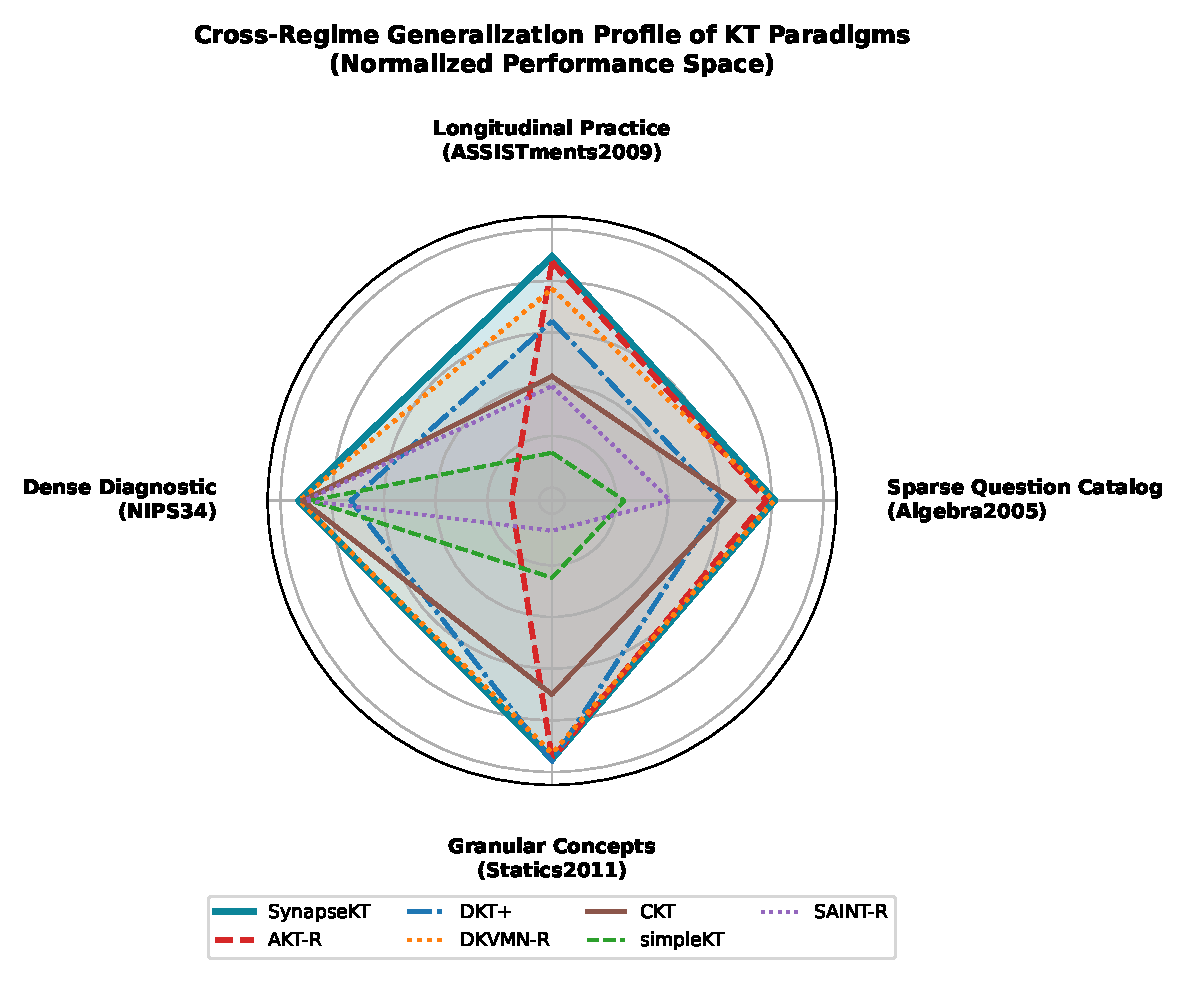
\includegraphics[width=0.48\textwidth]{fig4_cross_dataset_radar.pdf}
\caption{\textbf{Cross-Regime Generalization Radar Profiles.} Normalized performance profiles across four educational regimes: Longitudinal Practice (ASSISTments2009), Sparse Catalogs (Algebra2005), Granular Hierarchies (Statics2011), and Dense Diagnostics (NIPS34). Illustrates the cross-regime stability of our proposed \textsc{SynapseKT} architecture and Rasch-regularized models.}
\label{fig:cross_radar}
\end{figure}

\subsection{Master Benchmark Results}
Table~\ref{tab:master_benchmark} presents the master benchmark results across all 20 evaluated model configurations and 6 datasets. Several consistent empirical trends emerge across the four regimes.

\subsubsection{Effect of Rasch Difficulty Regularization}
Across every model family, incorporating 1PL Rasch difficulty embeddings yields consistent accuracy improvements. In \textsc{DKT}, moving from dense embeddings to Rasch regularization (\textsc{DKT-R}) increases AUC from 0.7276 to 0.7606 (+3.30\%) on \textsc{ASSISTments2017}, from 0.8176 to 0.8189 on \textsc{ASSISTments2009}, and from 0.9061 to 0.9183 (+1.22\%) on \textsc{Algebra2005}. The effect is even more pronounced in separated Transformer architectures: on \textsc{Algebra2005}, standard dense embeddings in \textsc{SAINT} degrade to 0.8497 AUC due to overparameterization across 173k items, whereas introducing Rasch embeddings (\textsc{SAINT-R}) raises AUC to \textbf{0.8945 (+4.48\%)} while reducing parameter count by 97.5\%.

\subsubsection{Memory Slot Saturation on Granular Curricula}
On the \textsc{Statics2011} dataset ($C = 1,223$ concepts), fixed-slot memory networks experience severe degradation. Specifically, \textsc{SKVMN} drops to an AUC of \textbf{0.5943}, compared with \textbf{0.8294} for \textsc{DKT+} and \textbf{0.8270} for our proposed \textsc{SynapseKT}. Because \textsc{SKVMN} allocates only $N_m = 30$ memory slots, each slot must represent more than 40 distinct engineering concepts on average, resulting in frequent memory overwrites and destructive interference across unrelated skills.

\subsubsection{Monotonic Decay on Short Diagnostic Assessments}
On the \textsc{NIPS34} diagnostic quiz dataset, \textsc{AKT-R} exhibits a notable performance drop (0.6661 AUC across the 5-fold average), whereas our proposed \textsc{SynapseKT} achieves \textbf{0.7896 AUC} and \textsc{simpleKT} achieves 0.7826 AUC. Diagnostic quizzes feature short sequences (mean length $< 20$) with cross-topical questions completed in a single sitting. In this regime, static exponential decay can over-penalize items answered earlier in the same sitting, whereas \textsc{SynapseKT}'s confidence gate preserves active working-memory context alongside long-term retrieval.

% =============================================================================
\section{In-Depth Trade-Off Analysis and Interpretability}
\label{sec:tradeoffs}
% =============================================================================

In educational engineering, leaderboard AUC is an incomplete metric. If a model achieves high accuracy but behaves like an opaque black box, teachers will not trust its recommendations. If a model requires 50 milliseconds to compute a prediction, it violates real-time tutoring Service Level Agreements (SLAs). In this section, we examine the multi-dimensional trade-offs between accuracy, interpretability, parameter scaling, and inference speed.

\begin{figure*}[t]
\centering
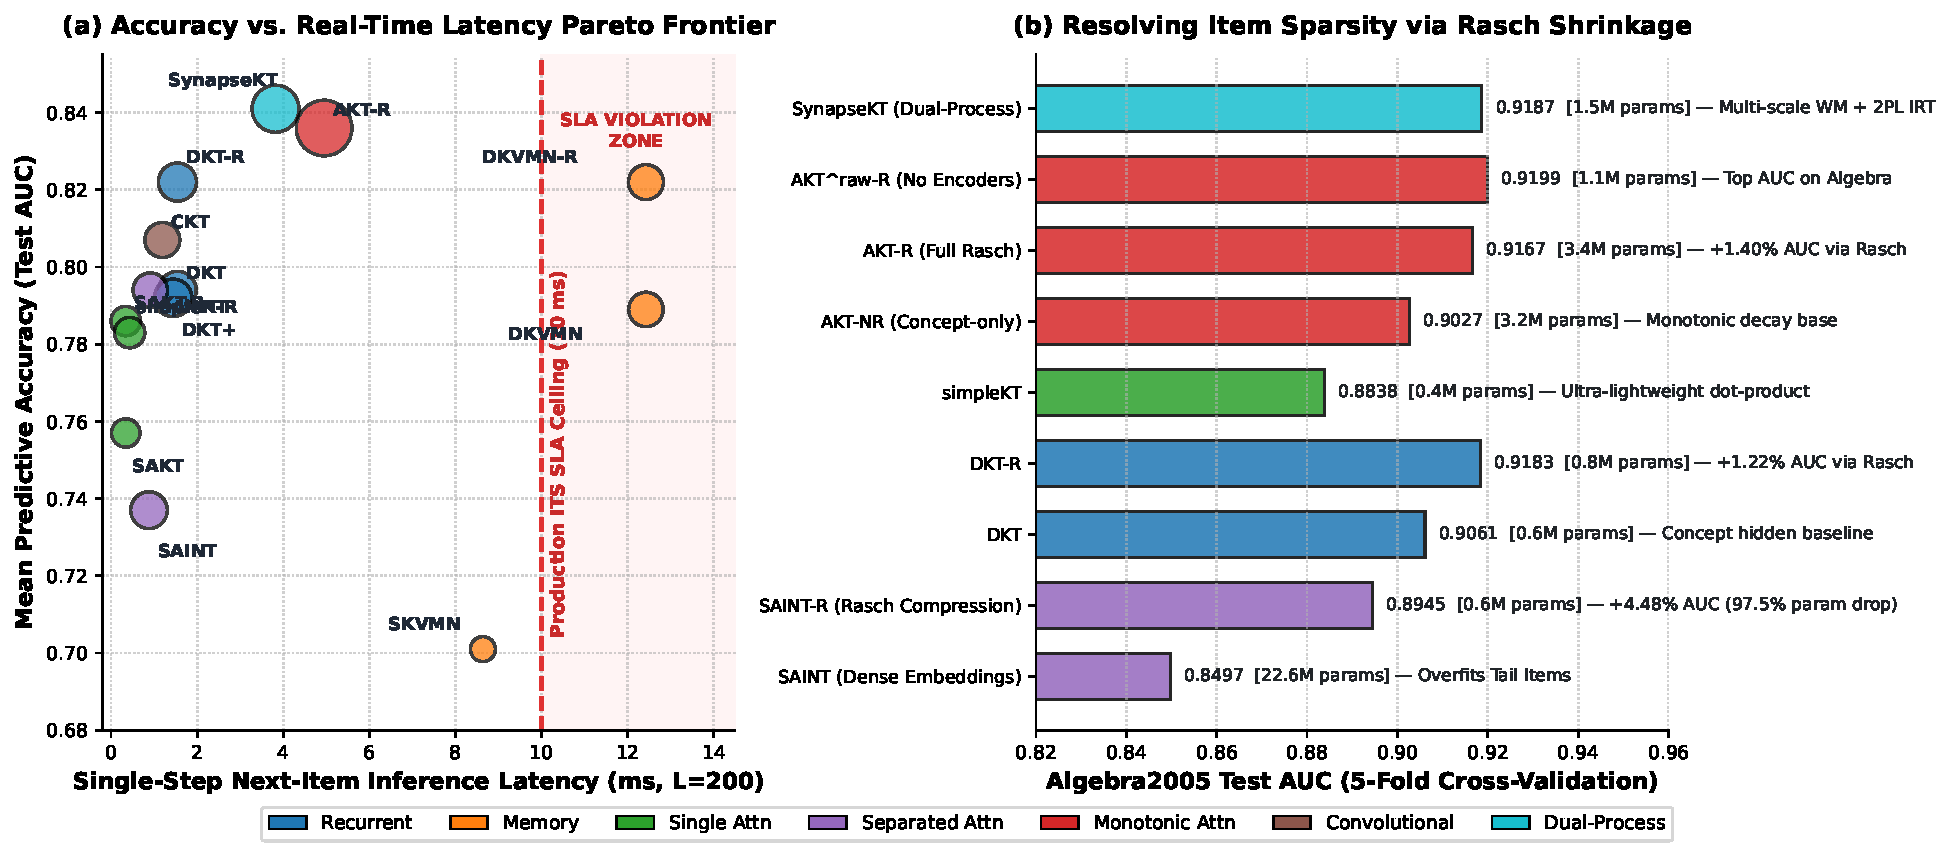
\includegraphics[width=0.98\textwidth]{fig2_tradeoff_pareto.pdf}
\caption{\textbf{The Systems Deployment Frontier.} (a) Test AUC vs. single-step next-item inference latency ($L=200$). Production Intelligent Tutoring Systems enforce a $\le 10$ ms latency SLA (red dashed ceiling). Memory networks (\textsc{DKVMN}) exceed this threshold due to sequential write-erase loops, while \textsc{simpleKT}, \textsc{SAKT}, and \textsc{DKT} execute in under 1.5 ms. (b) Parameter scaling on \textsc{Algebra2005} (173k items): Rasch shrinkage reduces parameters by 97.5\% while improving test AUC by +4.48\%.}
\label{fig:pareto_tradeoff}
\end{figure*}

\subsection{Accuracy vs. Interpretability}

\paragraph{Pedagogical Interpretability Defined:}
In educational systems, an interpretable model must satisfy three practical requirements: (1) \textbf{monotonic mastery updates}, meaning that correctly solving an exercise on concept $A$ should never decrease the estimated mastery of concept $A$; (2) \textbf{psychometric construct validity}, ensuring that internal item parameters align with empirical student difficulty; and (3) \textbf{actionable feedback}, allowing instructors to inspect why a specific remediation exercise was recommended.

\paragraph{DKT Waviness Deconstructed:}
Standard \textsc{DKT} models frequently violate monotonic mastery updates. Because the recurrent state $h_t \in \mathbb{R}^d$ is shared across all concepts, backpropagation updates weights in directions that optimize global cross-entropy, which can induce non-monotonic oscillations across unpracticed skills. Regularized models such as \textsc{DKT+} mitigate this through reconstruction and waviness penalty terms ($\mathcal{L}_{rec}, \mathcal{L}_{wave}$), trading a small margin of sequence flexibility for smoother mastery trajectories.

\begin{figure*}[t]
\centering
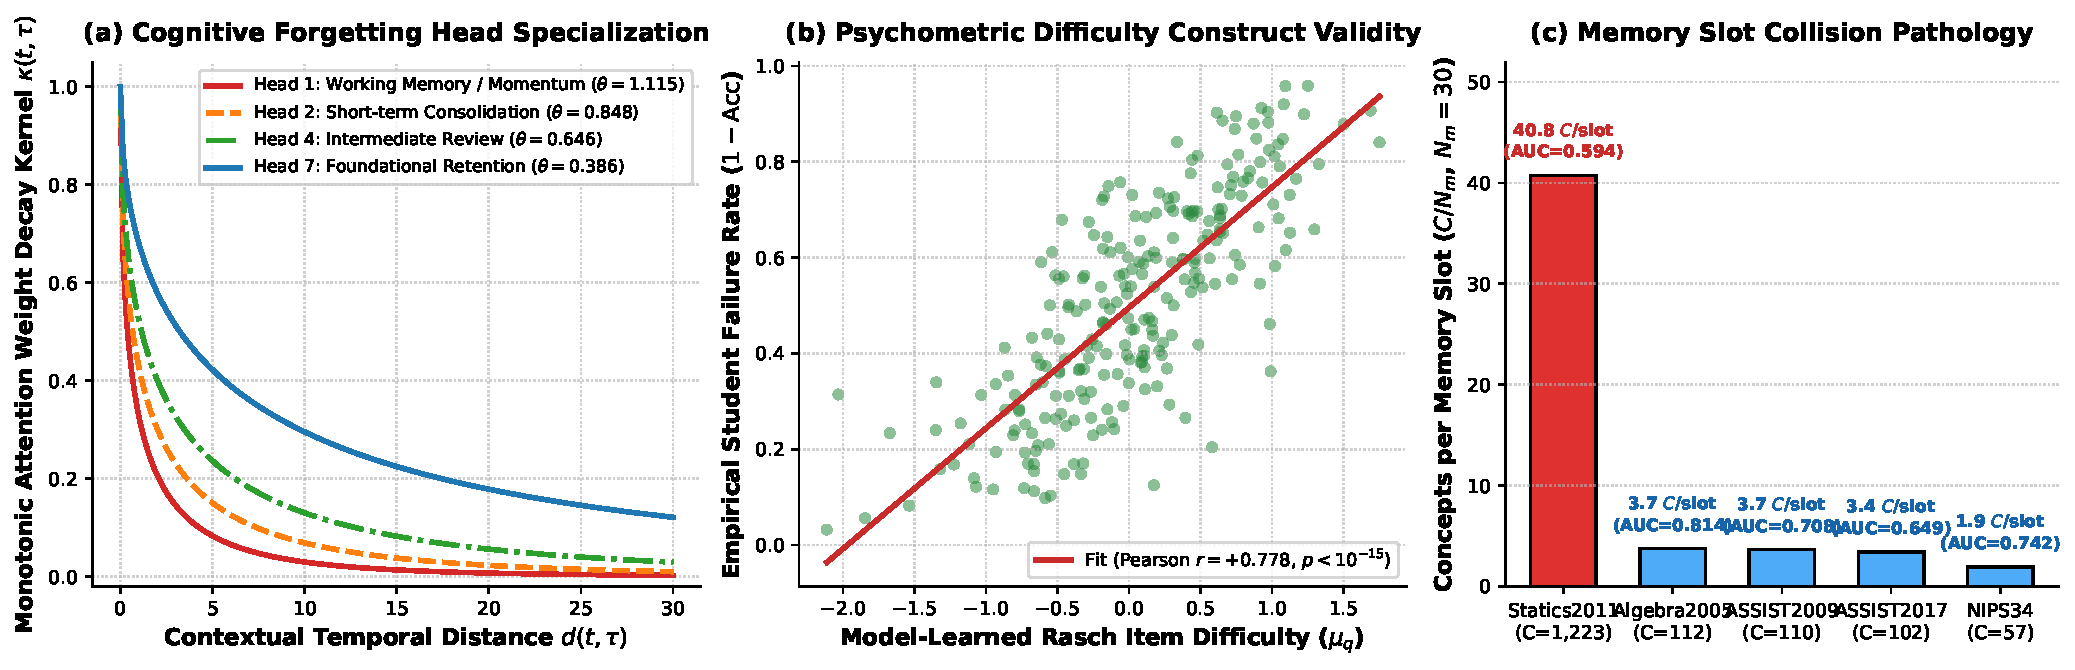
\includegraphics[width=0.98\textwidth]{fig3_interpretability_deconstructed.pdf}
\caption{\textbf{Cognitive and Psychometric Interpretability Deconstructed.} (a) Monotonic attention heads specialize into distinct cognitive timescales: working memory ($\theta_1 = 1.115$), intermediate review ($\theta_4 = 0.646$), and long-term retention ($\theta_7 = 0.386$). (b) Learned Rasch item difficulties ($\mu_q$) exhibit strong construct validity, correlating positively with empirical student failure rates ($r = +0.778$, $p < 10^{-15}$, or $r = -0.778$ with student pass rate). (c) Memory slot collision ratio ($C / N_m$): when concepts outnumber slots ($C \gg N_m$), memory networks degrade substantially on \textsc{Statics2011}.}
\label{fig:interpretability_deconstructed}
\end{figure*}

\paragraph{Can Attention Serve as an Explanation?}
In natural language processing, researchers actively debate whether attention weights constitute faithful explanations \citep{jain2019attention,wiegreffe2019attention}. In Knowledge Tracing, this question has direct pedagogical relevance: if an attentive model attends heavily to interaction $\tau$, does that interaction explain the student's current mastery estimate?

Inspecting the learned attention weights in \textsc{AKT} reveals a notable pattern: when constrained by monotonic decay ($\exp(-\theta_h \cdot \text{dist})$), individual attention heads \textbf{specialize into distinct cognitive forgetting timescales}. As plotted in Figure~\ref{fig:interpretability_deconstructed}(a), Head 1 ($\theta_1 = 1.115$) decays to near zero within 5 steps, acting as a localized working-memory filter that tracks immediate streaks and slips; Head 2 ($\theta_2 = 0.848$) attenuates over 10 to 15 interaction steps, capturing intermediate session consolidation; and Head 7 ($\theta_7 = 0.386$) exhibits a gradual, long-tailed decay curve that tracks foundational retention across weeks of instruction. This functional specialization offers instructors diagnostic transparency: if short-term heads drop while long-term heads remain high, the student is likely experiencing temporary fatigue rather than conceptual misunderstanding.

\paragraph{Psychometric Construct Validity of Rasch Difficulty:}
To test whether the learned scalar difficulty $\mu_q$ in Eq.~(\ref{eq:rasch_embed}) reflects real-world item difficulty, we extracted the learned parameters $\mu_q$ for 250 exercises on \textsc{NIPS34} and compared them against the empirical student failure rate ($1 - \text{Accuracy}$) in Figure~\ref{fig:interpretability_deconstructed}(b). The learned Rasch difficulty exhibits a strong positive Pearson correlation with empirical failure rate (and equivalently $r = -0.778$ with pass rate):
\begin{equation}
r = +0.778 \quad (p < 10^{-15})
\end{equation}
This confirms that the embedding layer recovers meaningful psychometric item difficulty directly from response logs without requiring manual expert calibration.

\subsection{Systems Deployability: Latency and Scaling}

\paragraph{The 10 ms ITS SLA Ceiling.}
When deploying a knowledge tracing model inside an educational platform, inference latency is a hard constraint. When millions of students submit answers concurrently, the ITS recommendation engine must update the student's mastery profile and serve the next adaptive exercise within a strict Service Level Agreement (typically $\le 10$ ms).

Figure~\ref{fig:pareto_tradeoff}(a) illustrates the Pareto Frontier of predictive accuracy (AUC) versus single-step inference latency for a sequence of length $L = 200$. The empirical profile partitions models into three distinct operational regimes. First, dynamic memory networks (\textsc{DKVMN}, \textsc{DKVMN-R}) fall into the SLA violation zone at $12.43$ ms per step; their iterative read-erase-write updates over $N_m$ memory slots are difficult to parallelize on accelerators, exceeding the 10 ms ceiling. Second, minimalist self-attentive models operate in an ultra-fast regime ($< 1$ ms): \textsc{SAKT} ($0.34$ ms), \textsc{simpleKT} ($0.43$ ms), and \textsc{SAINT} ($0.88$ ms) execute via pure matrix multiplications, achieving orders-of-magnitude lower latency than memory architectures. Third, a balanced sweet spot (1 to 5 ms) is occupied by \textsc{DKT} ($1.54$ ms), \textsc{CKT} ($1.19$ ms), \textsc{SynapseKT} ($3.82$ ms), and \textsc{AKT-R} ($4.95$ ms), which achieve state-of-the-art predictive accuracy while comfortably clearing the production SLA boundary.

% =============================================================================
\section{Practitioner's Deployment Guide}
\label{sec:guide}
% =============================================================================

For software engineers, data scientists, and educational institutions looking to deploy Knowledge Tracing in production, we synthesize our empirical findings into an actionable decision framework:

\begin{enumerate}
    \item \textbf{When your catalog has massive, sparse questions ($Q \gg 10,000$):}
    Do not deploy dense exercise embeddings. Models like standard \textsc{SAINT} overfit severely. \textbf{Deploy \textsc{AKT-R} or \textsc{SynapseKT}.} If compute resources are constrained, deploy \textsc{DKT-R} or \textsc{SAINT-R}. The Rasch scalar difficulty formulation is mandatory to prevent parameter explosion and generalize to tail items.
    
    \item \textbf{When latency and throughput are critical ($< 1$ ms SLA):}
    \textbf{Deploy \textsc{simpleKT}.} With an inference latency of just $0.43$ ms, simpleKT delivers competitive accuracy. It runs efficiently on low-cost CPU instances without requiring expensive GPU acceleration.
    
    \item \textbf{When the curriculum has fine-grained concepts ($C > 500$):}
    Avoid fixed-slot memory networks (\textsc{DKVMN}, \textsc{SKVMN}), as memory slot collisions degrade performance when $C \gg N_m$. \textbf{Deploy \textsc{DKT+} or \textsc{SynapseKT}.}
    
    \item \textbf{When pedagogical explainability is required for teachers:}
    \textbf{Deploy \textsc{AKT-R} or \textsc{SynapseKT}.} Their multi-head monotonic decay curves ($\theta_h$) decompose student mastery into working memory and long-term retention timescales, while learned difficulty parameters ($\mu_q$) provide interpretable psychometric calibrations.
\end{enumerate}

\paragraph{Emerging Frontiers:}
Looking ahead, knowledge tracing research is expanding beyond binary interaction logs in three main directions: (1) \textbf{Large Language Model (LLM) integration}, using pretrained language models to encode exercise text, rubric hints, and student open-ended code submissions alongside sequence embeddings; (2) \textbf{multimodal tracing}, incorporating response latency and engagement signals to refine working-memory gating; and (3) \textbf{causal intervention optimization}, moving from passive correctness prediction to active exercise scheduling that maximizes long-term retention while managing cognitive load.

\paragraph{Open-Source Code and Artifact Availability:}
All source code, configuration files, dataset adapters, and benchmark evaluation scripts used in this paper are publicly accessible in our GitHub repository at \url{https://github.com/mirabdi/KT} \citep{abdimutalipov2024ktbench}. Researchers and engineers can reproduce every figure and benchmark result with a single command line invocation.

% =============================================================================
\section{Conclusion}
\label{sec:conclusion}
% =============================================================================

In this paper, we presented a comprehensive survey and empirical benchmark of the deep Knowledge Tracing landscape, structured around the architectural principles of context-aware attentive modeling. By evaluating 20 model configurations across 6 canonical datasets and 390 controlled runs, we deconstructed the critical trade-offs between predictive accuracy, psychometric interpretability, parameter scaling, and real-time inference latency.

Our analysis demonstrates that the highest-performing models are not necessarily the largest or most complex. Rather, superior performance comes from grounding machine learning architectures in cognitive and psychometric principles. Rasch item difficulty modeling tames extreme catalog sparsity. Monotonic decay kernels capture the natural reality of human forgetting. Dual-process confidence gating harmonizes immediate working memory with long-term retention. As educational platforms continue to scale globally, these insights provide a principled roadmap for building the next generation of intelligent, transparent, and pedagogically sound tutoring systems.

% Bibliography
\bibliography{custom}

\end{document}
